\section{Values as Salience Priors: A Formal Account}\label{sec:formal}

%% ~3500 words / ~4–5 pages. Heaviest, most technical section.
%% Anchors: friston2015ActiveInferenceEpistemic, hesp2021DeeplyFelt,
%%   feldmanFriston2010Attention, parrFriston2017Attention,
%%   parrFriston2019AdvancedAtt, parviziWayne2024PreferencesAttention,
%%   limanowskiFriston2018Dark, torresan2025ShapeC, millidge2021EFE,
%%   ransom2020Cognition, veissiere2020TTOM, albarracin2022EpistemicCommunities,
%%   albarracin2025SocialPower, constant2019Regimes, heins2024CollectiveSurprise,
%%   heins2025AsOneAndMany, vasil2020SameKind, henrichGilWhite2001Prestige,
%%   henrich2009CREDs, chudek2012BystanderGaze, koster2022SillyRules.
%% Defensive: millidge2021EFE in a footnote.

\subsection{Attention is precision; salience is expected information gain}
\label{sec:attention-vs-salience}

The first step is to refuse a conflation that even active-inference researchers
routinely commit. \citet{feldmanFriston2010Attention} establish the load-bearing
identification: \emph{attention} is the inference of precision $\Prec$ on
prediction errors --- a gain on the likelihood mapping that determines which
channels of current sensory evidence dominate posterior updating. Higher
precision at a level of the hierarchy means a louder error signal at that
level, and louder errors do more work in revising beliefs. Salience is a
different quantity. \citet{parrFriston2017Attention,parrFriston2019AdvancedAtt}
draw the distinction with full formality: salience is the \emph{expected
information gain} associated with a candidate sample of the world ---
prospective and policy-conditional, not retrospective and stimulus-bound. To a
first approximation, attention is precision over the data the agent is
\emph{currently} consuming; salience is a forward-looking quantity that scores,
for each candidate next observation, how much the agent's posterior would
contract were that observation actually obtained.\footnote{We will write the
salience operator $\salience$ informally as ``expected information gain'' and
will not commit to the full expected-free-energy decomposition. The logical
content of our argument requires only that preferences and information gain
appear additively in a single objective; we do not require that the
expected-free-energy functional be uniquely derivable in the sense of
\citet{millidge2021EFE}, whose foundational concerns about EFE we acknowledge
but do not need to resolve here.} Salience is therefore not a property of the
distal world. It is a property of the prior-shaped uncertainty landscape an
agent carries around with it.

The framing matters because, once one allows that deep priors set the precision
weights distributed across the hierarchy, salience inherits its shape from
those priors. \citet{parviziWayne2024PreferencesAttention} makes the point most
forcefully: under active inference, the endogenous--exogenous attention
dichotomy collapses. There is no precision-free signal entering the cognitive
system. What looks like bottom-up, stimulus-driven capture is in fact the
allocation of precision against prediction errors generated by deep generative
expectations the agent already holds. The corollary, due to
\citet{limanowskiFriston2018Dark}, is that phenomenal transparency and opacity
are themselves precision phenomena --- when precision on a level is high and
stable, the agent ``sees through'' it; when precision is low or unsettled, the
level itself becomes available to introspection. Together, these results
license the move at the heart of this paper: \emph{deep priors --- including
the agent's preferences --- shape what becomes salient}. \citet{ransom2020Cognition}
press the strongest empirical objection to attention-as-precision: affect-biased
attention orients the system toward emotionally significant stimuli even when
their feature-level precision is low. We engage this directly because it is
not in fact a counter-example. Their data are consistent with a deep-priors-set-
precision rebuttal: emotionally significant stimuli are exactly the ones for
which the agent has high-precision priors over their value-relevance, and
those high-precision deep priors propagate down the hierarchy as gain
modulation on the lower-level error signals that constitute affect-biased
attention. The Ransom et al.\ result, in other words, is evidence \emph{for}
the framing this paper develops, provided one is willing to grant that values
sit upstream of sensory precision-setting --- which is exactly the move we now
make.

\subsection{Values as prior preferences $\C$}
\label{sec:values-as-C}

Active inference furnishes a single object that does the work of
``preferences,'' ``goals,'' ``values,'' and ``utility'' in a unified register.
The prior preference distribution $\C$ encodes the agent's expectations about
\emph{which observations} it will tend to obtain. Crucially, these are
expectations in the ordinary Bayesian sense: $\C$ is a prior over outcomes,
and the agent acts in such a way as to make its sensory experience consistent
with this prior \citep{friston2015ActiveInferenceEpistemic}. ``Wanting'' an
outcome and ``expecting'' it become two faces of one variational quantity.
\citet{friston2015ActiveInferenceEpistemic} establish the formal apparatus that
puts pragmatic value (the expected log-probability of preferred outcomes) and
epistemic value (expected information gain about hidden states) into a single
additive objective; preferences and salience appear as commensurable terms,
not as separate cognitive systems. Importantly, our argument requires only the
\emph{decomposition} --- preferences and information are summed in a single
currency --- and not the strong claim that this currency is uniquely fixed by
expected free energy.

The bridge from values-as-priors to precision is supplied by
\citet{hesp2021DeeplyFelt}. They formally identify valence with the
\emph{expected precision of the action model}: a positively valenced state of
affairs is one in which the agent expects its model to reliably support
goal-directed action; a negatively valenced one is one in which it expects
that model to be unreliable. ``Caring about'' an outcome, on this account, is
\emph{having a high-precision prior expectation of obtaining it}. This is
the move that turns the abstract notion of $\C$ into a precision-bearing
object. A community that shares values is a community whose members hold
similarly shaped, similarly precise $\C$'s --- and, by the result of
\S\ref{sec:attention-vs-salience}, a community whose members find the same
features of the world salient.

\begin{definition}[Values as prior preferences]
\label{def:values}
An agent's \emph{values} over outcomes are encoded as the prior preference
distribution $\C$ in its generative model. The valence of an outcome $\obs$ is
$\log p(\obs \mid \C)$; high-precision $\C$ expresses sharp values and
low-precision $\C$ expresses diffuse values. Equivalently, a value is a
high-precision prior expectation of observing a class of outcomes, and the
felt strength of a value is the precision of that expectation.
\end{definition}

This definition has two immediate consequences. First, it dissolves the
intuitive contrast between ``what an agent wants'' and ``what an agent
expects'': both are encoded by $\C$, and the dual reading is constitutive of
the active-inference account, not a translation artefact. Second, it makes
``valuing'' a graded property: there is no all-or-nothing distinction between
having and not having a value, only the continuous question of how peaked
$\C$ is over an outcome class. \citet{constant2019Regimes} extend this picture
to the social register by introducing \emph{deontic value}: a third value
type alongside epistemic and pragmatic, expressed as policy priors cued by
environmentally and socially supplied scripts. Deontic cues (a red traffic
light, a raised eyebrow, an averted gaze) emerge from repeated collective
behaviour and reify cultural-group preferences as Bayes-optimal action
defaults. Deontic priors are policy-level priors --- priors over what to do
given a cue --- whereas $\C$ is an outcome-level prior. The two layers
interact: outcome-level preferences shape which policies look pragmatically
valuable, and deontic policy priors shape which policies get selected without
explicit deliberation. Section~\ref{sec:installation} formalises how the
outcome-level layer, $\C$, is itself acquired from a community.

\subsection{The $\C$-installation channel}
\label{sec:installation}

The genuinely new piece of formal machinery this paper supplies concerns how
$\C$ is \emph{installed}. Existing accounts treat $\C$ as exogenously
specified by the modeller. We propose instead that $\C$ is acquired from a
community, by a precision-modulated channel from observed-other-behaviour into
the agent's own preference distribution. Schematically:
\begin{equation}
\label{eq:channel}
\text{community behaviour} \;\xrightarrow{\;\;\;\salience \cdot \prc\;\;\;}\;
\text{updated } \C,
\end{equation}
where $\prc$ is a scalar channel precision and $\salience$ is the salience
allocated to the observed behaviour. The channel is bidirectional in the
deeper sense that its input $\salience$ is itself determined by the agent's
current $\C$ (via \S\ref{sec:attention-vs-salience}); the agent's existing
preferences shape which conspecific behaviours it samples and weighs, and the
samples it weighs shape its updated preferences. Equation~\eqref{eq:channel}
is therefore not a one-shot transmission rule but the elementary step of a
fixed-point dynamic which we describe in \S\ref{sec:loop}.

The empirically novel claim is that prestige cues and credibility-enhancing
displays --- the documented mechanisms of human cultural transmission ---
function as modulators of the channel precision $\prc$, not as content
priors. \citet{henrichGilWhite2001Prestige} establish prestige as
freely-conferred deference: high-prestige individuals are not coerced into
attention-monopoly but selected for it by observers as a heuristic for
locating skilled or successful models. \citet{henrich2009CREDs} argues that
costly displays of commitment to beliefs and norms function as honest signals
that increase observers' willingness to acquire those beliefs and norms.
Both mechanisms have been treated in cultural-evolutionary theory as
\emph{biases on what to copy}; we propose they are better treated as
modulators of \emph{how strongly to update} on observation, that is, as gains
on $\prc$. The empirical anchor for this reframing is
\citet{chudek2012BystanderGaze}, whose experimental finding has been
under-exploited in the active-inference literature. Children observed
multiple potential models, with bystanders' gaze biased toward one of them.
Children subsequently preferred to copy the bystander-attended model across
\emph{multiple} content domains --- not just the domain in which the
bystander gaze occurred. This generality is the formal signature of a
precision parameter rather than a content prior: a content prior would
predict transfer only to similar contents, while a generalised precision
parameter predicts transfer across the whole channel through which content
flows. Bystander gaze, on this reading, is a CRED-like cue whose mechanistic
effect is to elevate $\prc$ on the channel from the attended model into the
observer's $\C$.

This reading must be distinguished from two adjacent accounts.
\citet{veissiere2020TTOM}'s Thinking Through Other Minds framework treats
culture as installing \emph{regimes of attention} --- shared styles of
allocating attentional resources that mark some channels as reliable. TTOM
operates at the level of shared generative-model structure and the precision
weights that style channel reliability; it is silent on the content of $\C$.
\citet{vasil2020SameKind} argue that human communication is enabled by a
deep prior that one's interlocutor is the ``same kind of creature'' as
oneself, licensing rapid alignment of generative models. This is also a
structural prior, not a content prior. We do not take issue with either
account; we extend them. The TTOM regime determines \emph{whose} $\C$ a
learner samples; the same-kind prior makes that sampling possible at all;
prestige and CRED cues then determine \emph{how much} the sampled
behaviour is allowed to modify the learner's $\C$. The channel of
Equation~\eqref{eq:channel} formalises the third move, which the prior
literature gestures at without naming. Differentiation from
\citet{albarracin2025SocialPower} requires special care, since their account
is the closest existing neighbour. They formalise social power as the
differential capacity to set policy-precision (often denoted $\alpha$) in
others' generative models. Power, on their account, sits at the
\emph{policy-precision} layer: empowered agents anchor others' policy priors
to their own outputs and benefit from the resulting attention asymmetry. Our
account sits at the \emph{prior-preference content} layer:
$\C$-installation modifies what others come to want, not which policies they
deploy in service of pre-given wants. The two layers are coupled --- a
community whose $\C$ has been installed by prestige cues will in addition
exhibit asymmetric policy-precision around the prestige-bearer --- but they
are formally separable, and our claim is that the $\C$-content channel is
the one cultural evolution has been describing for half a century without
naming it as such.

\subsection{The fixed-point loop}
\label{sec:loop}

The four moves --- values are $\C$ (\S\ref{sec:values-as-C}); $\C$ shapes
salience via precision (\S\ref{sec:attention-vs-salience}); salience directs
copying through the prestige/CRED-modulated channel (\S\ref{sec:installation});
copying installs $\C$ in the next-generation agent --- close into a loop.
Figure~\ref{fig:loop} renders the loop graphically.

\begin{figure}[t]
\centering
%% Manual TikZ positioning is used here for pdfLaTeX compatibility.
%% A `graphs`+`graphdrawing` (layered/circular) version is available but
%% requires LuaLaTeX; the manual layout below produces a clean circular
%% diagram under either compiler.
\begin{tikzpicture}[
  >=Stealth,
  node distance=18mm,
  every node/.style={font=\small},
  prior/.style={draw=blue!70!black, fill=blue!8, thick, rounded corners,
                inner sep=4pt, align=center, minimum width=24mm,
                minimum height=10mm},
  precision/.style={draw=orange!80!black, fill=orange!10, thick, rounded corners,
                    inner sep=4pt, align=center, minimum width=24mm,
                    minimum height=10mm},
  social/.style={draw=red!70!black, fill=red!8, thick, rounded corners,
                 inner sep=4pt, align=center, minimum width=24mm,
                 minimum height=10mm},
  arr/.style={->, thick}
]
  %% Five nodes arranged on a circle
  \node[prior]     (commC)   at ( 90:36mm) {community $\C$};
  \node[precision] (sal)     at ( 18:36mm) {salience\\landscape};
  \node[social]    (att)     at (-54:36mm) {attention \&\\copying};
  \node[social]    (channel) at (234:36mm) {prestige / CRED\\channel ($\prc$)};
  \node[prior]     (instC)   at (162:36mm) {installed $\C$\\(next agent)};

  %% Cycle arrows
  \draw[arr, blue!70!black]   (commC)   -- (sal);
  \draw[arr, orange!80!black] (sal)     -- (att);
  \draw[arr, red!70!black]    (att)     -- (channel);
  \draw[arr, red!70!black]    (channel) -- (instC);
  \draw[arr, blue!70!black]   (instC)   -- (commC);

  %% Inner gloss
  \node at (0,0) {\itshape fixed-point};
\end{tikzpicture}
\caption{The values-as-salience-priors loop. A community's prior preferences
($\C$) determine the salience landscape, which directs attention and copying
via prestige- and CRED-modulated channels; the resulting installed $\C$ in
next-generation agents reproduces (or shifts) the community-level prior.
Colours: blue = prior content; orange = precision (salience); red = social
channel.}
\label{fig:loop}
\end{figure}

The loop has three qualitatively distinct dynamical regimes. \emph{Convergence}
obtains when channel precision $\prc$ is high enough and prestige consensus
is sufficient that successive generations install $\C$'s closely matching
the community-level distribution; the loop reproduces the prior with high
fidelity, and norms are robust. \emph{Bifurcation} occurs when the loop
factorises across sub-populations whose internal $\prc$ exceeds the
cross-population $\prc$: \citet{albarracin2022EpistemicCommunities} demonstrate
this regime explicitly with their epistemic-community simulations, in which
shared priors over source reliability lock sub-communities into echo-chamber
attractors that resist cross-community correction. \emph{Dissolution} occurs
when $\prc$ collapses across the whole community --- when prestige cues lose
their force, CRED bearers are absent or distrusted, or the salience
landscape becomes too noisy to support coherent copying --- and the
community-level $\C$ flattens, as norms lose precision and content drifts.
A subtle but important point follows from \citet{heins2025AsOneAndMany}: the
community-level $\C$ is \emph{not} simply the average of individuals' $\C$'s.
Group-level generative models of a coupled collective have non-trivial
emergent structure, and the equilibrium behaviour of the loop in
Figure~\ref{fig:loop} is a property of the coupled system, not a moment of
the individual-level distribution. We adopt this caution: when we speak of
``the community's $\C$,'' we mean the aggregate that emerges from the loop
dynamics, not a population mean.

\subsection{Norms as stabilised regions of high-precision shared $\C$}
\label{sec:norms}

The loop dynamics give us a precise formulation of what norms are. A norm is
not a rule, an equilibrium, or a piece of representational content per se;
it is a region of outcome space where the community's $\C$ has both high
mass and high precision, stabilised by the loop of
\S\ref{sec:loop}.

\begin{definition}[Norm]
\label{def:norm}
A \emph{norm} in a community is a region $\norm \subseteq \mathcal{O}$ of
outcome space such that the community-level prior preference distribution
has both high mass on $\norm$ and high precision around $\norm$, where the
precision is sufficient that observed deviations from $\norm$ generate
prediction errors strong enough to drive both perception (the violation
\emph{feels} wrong) and action (correction, sanction, or attention-withdrawal).
\end{definition}

The definition recovers and explains three otherwise puzzling features of
norms. First, it explains why \emph{violations of norms feel surprising in a
way that violations of mere regularities do not}: high-precision priors over
$\C$ generate large prediction errors when violated, and high-precision
errors are exactly what valenced surprise consists of
\citep{hesp2021DeeplyFelt}. Second, it explains the ``silly rules'' result of
\citet{koster2022SillyRules}, where adding arbitrary content-free taboos
into a multi-agent reinforcement-learning environment improves agents'
acquisition of welfare-relevant norms. Under our account, what silly rules
do is pump up the precision of the meta-prior ``a normative regime is in
operation'' without committing to particular content; once that precision is
elevated, agents acquire welfare-relevant norms faster because the
$\C$-installation channel is opened wider. The mechanism Köster et al.\
identify is exactly the precision-modulator move of \S\ref{sec:installation},
written in MARL form. Third, the definition makes contact with the
deontic-value apparatus of \citet{constant2019Regimes}: norms-as-regions of
high-precision $\C$ generate the environmental and social cues that, in a
mature normative culture, become deontic priors over policies.
Outcome-level $\C$ and policy-level deontic priors thus stand in a
relationship that the active-inference literature already supports: deontic
cues short-circuit pragmatic deliberation when the loop has stabilised the
underlying $\C$, allowing norm-following to occur as Bayes-optimal action
under environmentally cued priors. \citet{heins2024CollectiveSurprise}
furnish the closest existing demonstration that norm-like collective
patterns can emerge from agents minimising variational free energy under
coupled generative models, without explicit social-force or utility rules.
Our claim is that the same logic, applied to the prior-preference content
layer rather than the kinematic state layer, recovers the cultural-norms
regime.

\subsection{The shape of $\C$: sharp, broad, and shaped}
\label{sec:shape-of-C}

Norms differ in more than location. They differ in the \emph{shape} of $\C$
they instantiate. \citet{torresan2025ShapeC} provide the empirical
demonstration that drives this subsection: in a grid-world navigation task,
they compare four parameterisations of $\C$ --- hard goals (delta-like
peaked priors), soft goals (broad priors), and either of these with or
without intermediate goal shaping. Their finding has direct consequences for
our account of norms.

\begin{figure}[t]
\centering
%% Three-panel PGFPlots figure laid out via \pgfplotsset groupplots-style
%% positioning would require an extra \usepgfplotslibrary{groupplots} in the
%% preamble; we instead use three independent axis environments arranged
%% horizontally inside a single tikzpicture, which works under the existing
%% pgfplots load in main.tex without further dependencies.
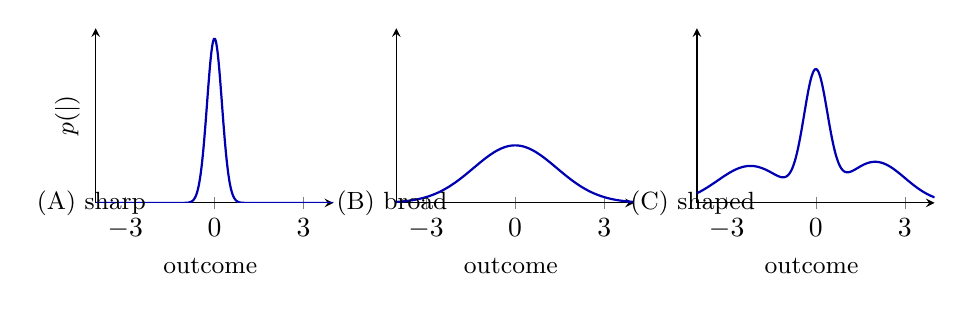
\begin{tikzpicture}
  \pgfplotsset{
    every axis/.append style={
      width=4.6cm, height=3.8cm,
      xmin=-4, xmax=4, ymin=0, ymax=0.85,
      xtick={-3,0,3}, ytick=\empty,
      axis lines=left,
      every axis label/.style={font=\footnotesize},
      every axis title/.style={font=\small},
    }
  }
  \begin{axis}[
    name=panA, at={(0,0)}, anchor=south west,
    xlabel={\small outcome $\obs$}, ylabel={\small $p(\obs\mid\C)$},
    title={\small (A) sharp $\C$}
  ]
    \addplot[thick, blue!70!black, smooth, samples=200, domain=-4:4]
      {0.8*exp(-((x-0)^2)/(2*0.25^2))};
  \end{axis}
  \begin{axis}[
    name=panB, at={(panA.south east)}, anchor=south west, xshift=8mm,
    xlabel={\small outcome $\obs$},
    title={\small (B) broad $\C$}
  ]
    \addplot[thick, blue!70!black, smooth, samples=200, domain=-4:4]
      {0.28*exp(-((x-0)^2)/(2*1.4^2))};
  \end{axis}
  \begin{axis}[
    name=panC, at={(panB.south east)}, anchor=south west, xshift=8mm,
    xlabel={\small outcome $\obs$},
    title={\small (C) shaped $\C$}
  ]
    \addplot[thick, blue!70!black, smooth, samples=200, domain=-4:4]
      {0.6*exp(-((x-0)^2)/(2*0.4^2))
       + 0.2*exp(-((x-2)^2)/(2*1.0^2))
       + 0.18*exp(-((x+2.2)^2)/(2*1.1^2))};
  \end{axis}
\end{tikzpicture}
\caption{The shape of $\C$ governs the exploration--exploitation tradeoff
and the robustness of installed values. (A) Sharp $\C$: hard goals; fast
convergence; fragile to perturbation. (B) Broad $\C$: soft goals; preserved
exploration; slow drift. (C) Shaped $\C$: a peak with structured shoulders
on either side --- most performant per \citet{torresan2025ShapeC}; a hybrid
of pragmatic and epistemic value.}
\label{fig:shape}
\end{figure}

A sharp $\C$ (Figure~\ref{fig:shape}A) is a delta-like preference over a
narrow outcome region. Sharp priors push the expected-free-energy objective
toward pragmatic value at the expense of epistemic value: agents converge
fast on the preferred outcome but under-sample alternatives, fragility
follows, and small environmental perturbations that move the optimal action
off the prior's peak are not detected because the precision penalty on
sampling alternatives is large. A broad $\C$ (Figure~\ref{fig:shape}B) is a
diffuse preference covering many outcomes. Broad priors preserve epistemic
value but achieve slower convergence on any particular target; in the limit,
a perfectly flat $\C$ collapses the pragmatic term entirely, and the agent
becomes a pure information-seeker. A shaped $\C$ (Figure~\ref{fig:shape}C)
combines a sharp peak on a target outcome with structured residual mass on
neighbouring outcomes --- the goal-shaping regime
\citet{torresan2025ShapeC} identify as most performant. Shaped $\C$
preserves the pragmatic gradient toward the preferred outcome while
maintaining enough probability on alternatives to support continued
exploration.

The translation to norms is direct. A community whose shared $\C$ is sharp
is a community of strongly aligned values that converges fast and resists
perturbation poorly --- a fragility property of normative coherence that is
otherwise hard to articulate. A community whose shared $\C$ is broad
preserves exploration of normative alternatives but coordinates poorly. A
community whose shared $\C$ is shaped --- a peak of strong commitments
flanked by structured latitude --- combines the convergence properties of
the first with the robustness of the second. This maps onto a familiar
cultural-evolutionary observation: healthy traditions tend to combine sharp
core commitments with broad peripheral latitude, and the precision of $\C$
is graded across content rather than uniformly high. Definition~\ref{def:norm}
must be read in this light: a norm is a high-precision \emph{region}, not a
high-precision \emph{point}, and the shape of the surrounding gradient is a
substantive property of the norm with measurable consequences for the
loop's robustness.

\subsection{Synthesis}
\label{sec:formal-synthesis}

The four moves of this section close the gap identified in \S\ref{sec:cooperative-ai}.
Values are formally identified with the prior preference distribution $\C$
(Definition~\ref{def:values}); $\C$ is installed by a
prestige- and CRED-modulated precision channel from observed-other-behaviour
into the agent's own preferences (\S\ref{sec:installation}); norms are
stabilised regions of high-precision shared $\C$ in a community
(Definition~\ref{def:norm}), held in place by the fixed-point loop of
Figure~\ref{fig:loop}; and the shape of $\C$ governs the exploration--exploitation
balance and therefore the robustness of installed values
(\S\ref{sec:shape-of-C}). The community-to-$\C$ arrow that the literature
described without naming is now formal. It is also the arrow on which the
cooperative-AI implications of Section~\ref{sec:simulation} turn: a system that
mediates the prestige- and CRED-bearing channel mediates the precision of
the cultural-transmission machinery itself, with consequences for the
stability of human normative orders that we take up next.
